\documentclass[11pt]{article}
\usepackage{amsmath,amssymb,amsfonts,epsfig,algorithm,algorithmic,url}
\usepackage{tikz}
\usetikzlibrary{positioning}

\textheight 8.8truein
\parskip 0.1in
\topmargin -0.5truein
\textwidth 6.5truein
\oddsidemargin -0.05in
\evensidemargin -0.05in
% \renewcommand{\baselinestretch}{1.2}   %line space adjusted here
\setcounter{footnote}{0}
\sloppy

\renewcommand{\theequation}{\thesection.\arabic{equation}}
\newcommand{\newsection}{\setcounter{equation}{0}\section}

% redefining commonly used symbols
\DeclareMathOperator{\trace}{Tr}

\newtheorem{theorem}{Theorem}
\newtheorem{proposition}[theorem]{Proposition}
\newtheorem{lemma}[theorem]{Lemma}
\newtheorem{corollary}[theorem]{Corollary}
\newtheorem{definition}[theorem]{Definition}
\newtheorem{example}[theorem]{Example}

\begin{document}
\title{\bf Sampling Methods for Optimal Control}
\date{\today}
\author{Bolei Di}
%\normalsize{}
\maketitle
\begin{abstract}

\end{abstract}

\section{Basic Theory}\label{sec:intro}
This is the theorem that connects sampling to optimization.
\begin{gather*}
\min_x f(x) = \min_p E[f(x)]
\end{gather*}
Suppose that $f(x)$ reaches its minimum at $x^{\star}$, then one optimal distribution over $x$ is $p^{\star}(x)=\delta(x-x^{\star})$. 
Here we relax the stochastic optimization on the right side by adding a term that is the Kullback-Leibler divergence of $p(x)$ and another arbitrary distribution $q(x)$:
\begin{gather*}
\min_x f(x) = \min_p E[f(x)] \leq \min_p E[f(x)] + \lambda D_{KL}(p||q)
\end{gather*}
where $D_{KL}(p||q)=\int_x p(x) \ln \frac{p(x)}{q(x)} \text{d}x \geq 0$, which is always non-negative. 
The optimal solution to the relaxed problem has a simple, analytic form, surprisingly:
\begin{gather*}
p^{\star}(x) = \frac{1}{Z} e^{-\frac{1}{\lambda}f(x)} q(x)
\end{gather*}
where $Z$ is a normalizing factor. 
We can choose the arbitrary distribution $q(x)$ to be Gaussian and define $L(x)=e^{-\frac{1}{\lambda}f(x)}$, we can get:
\begin{gather*}
p^{\star}(x) = Z^{-1} L(x) \mathcal{N}(x)
\end{gather*}
For an optimal control problem, we can define the cost function $f(x)$ to be minimized in terms of the states and inputs $x$, hence we often have an analytic expression for $L(x)$. Then using the elliptical slice sampling technique we can generate random numbers following $p^{\star}(x)$ distribution. 

\section{Programming}
Controllers and systems are treated as instances of classes. Diagram of systems' classes and inheritance: \\

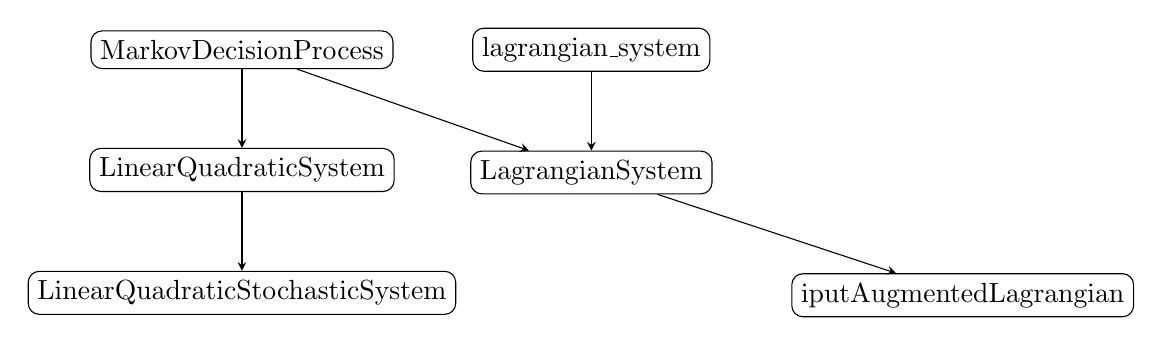
\begin{tikzpicture}[>=stealth,every node/.style={shape=rectangle,draw,rounded corners},]
	% create classes
    \node (MDP) {MarkovDecisionProcess};
	\node (LQS) [below = of MDP] {LinearQuadraticSystem};
	\node (LQSS) [below = of LQS] {LinearQuadraticStochasticSystem};
	\node (ls) [right = of MDP] {lagrangian\_system};
	\node (LS) [below = of ls] {LagrangianSystem};
	\node (iAL) [below right = of LS] {iputAugmentedLagrangian};	
	
%	\node () [] {};
     
	% indicates inheritance via connections
	\draw[->] (MDP) to (LQS);    
    \draw[->] (LQS) to (LQSS);
	\draw[->] (ls) to (LS);    
    \draw[->] (MDP) to (LS);
    \draw[->] (LS) to (iAL);
    
    %\draw[->] () to ();
    
\end{tikzpicture}

Diagram of controller classes and inheritance: \\

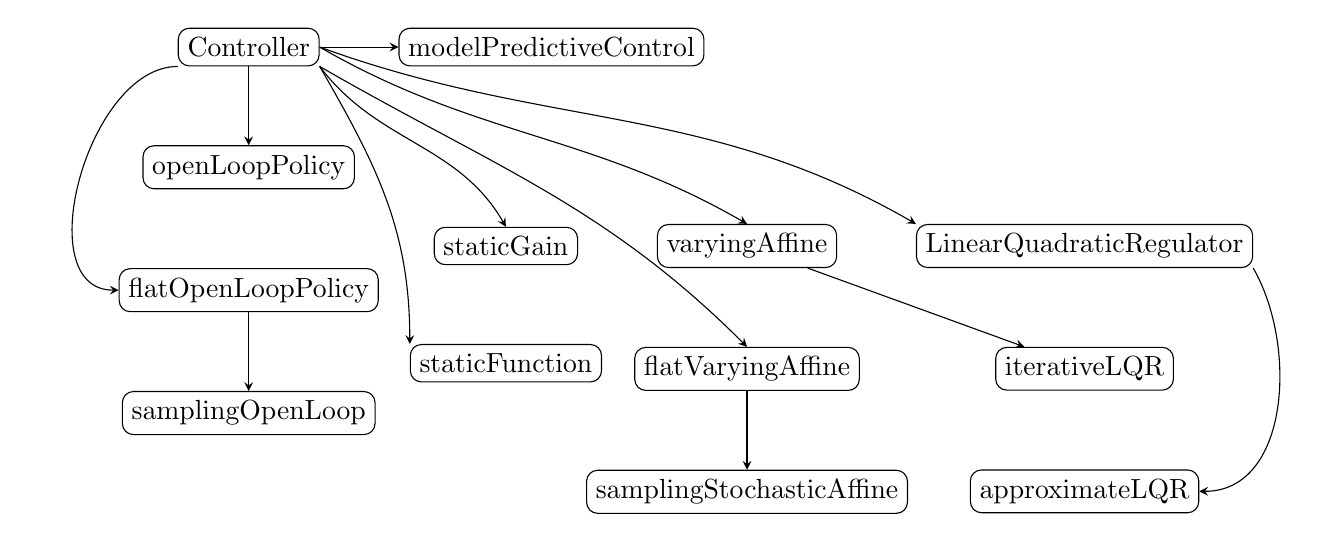
\begin{tikzpicture}[>=stealth,every node/.style={shape=rectangle,draw,rounded corners},]
	% create classes
    \node (con) {Controller};
	\node (oLP) [below = of con] {openLoopPolicy};
	\node (mPC) [right = of con] {modelPredictiveControl};	
	\node (fOLP) [below = of oLP] {flatOpenLoopPolicy};
	\node (sG) [right = of oLP,yshift = -1cm] {staticGain};
	\node (vA) [right = of sG] {varyingAffine};
	\node (fVA) [below = of vA] {flatVaryingAffine};
	\node (sF) [below = of sG] {staticFunction};
	\node (LQR) [right = of vA] {LinearQuadraticRegulator};
	\node (iLQR) [below = of LQR] {iterativeLQR};
	\node (aLQR) [below = of iLQR] {approximateLQR};
	\node (sOL) [below = of fOLP] {samplingOpenLoop};
	\node (sSA) [below = of fVA] {samplingStochasticAffine};
	
	%\node () [] {};
     
	% indicates inheritance via connections
	\draw[->] (con) to (mPC);
	\draw[->] (con.south west) to[out = 180, in = 180] (fOLP);
	\draw[->] (con.east) to[out = -30,in = 150] (vA.north);
	\draw[->] (con.south east) to[out = -53,in = 120] (sG.north);
	\draw[->] (con.east) to[out = -20,in = 150] (LQR.north west);
	\draw[->] (con.south east) to[out = -60,in = 90] (sF.north west);
	\draw[->] (con.south east) to[out = -30,in = 135] (fVA.north);
	\draw[->] (con) to (oLP);
	\draw[->] (vA) to (iLQR);
	\draw[->] (LQR.south east) to[out = -60,in = 0] (aLQR.east);
	\draw[->] (fOLP) to (sOL);
	\draw[->] (fVA) to (sSA);    
    
    %\draw[->] () to ();
    
\end{tikzpicture}


\end{document}
